\documentclass{article}
\usepackage{graphicx}
\usepackage[a4paper, margin=1in]{geometry}
\usepackage{hyperref}
\graphicspath{{assets/}}

\title{P2P Chat and VoIP Application using UDP in Java}

\author{
    \small Aristotle University of Thessaloniki - Department of Electrical and Computer Engineering \\[0.5em]
    \small Computer Networks II\\[1.5em]
    Epameinondas Bakoulas and Maria Sotiria Kostomanolaki \\[1em]
}

\date{December 2024}

\begin{document}

\maketitle

\begin{abstract}
This report presents the development of a Peer-to-Peer (P2P) Chat and Voice over IP (VoIP) application, created as part of the 
Computer Networks II course at Aristotle University of Thessaloniki. The application is built using Java's \texttt{java.net} 
library to manage network communications. 

The project demonstrates a deeper understanding of Internet Protocols (IP) by allowing users to switch between UDP and TCP protocols 
through a command. This feature highlights the trade-offs between speed and reliability in network communications. 
Additionally, cryptographic techniques are integrated to secure data exchanges, ensuring the privacy and integrity of communications.
\end{abstract}

\section {UDP Chat and VoIP Application}

\subsection{Variables}
The application uses two \texttt{DatagramSocket} objects:
\begin{itemize}
    \item \texttt{messageSocket} for handling message communication
    \item \texttt{voiceSocket} for handling voice data
\end{itemize}
This separation is important to avoid conflicts between the different types of data (text and voice) that are transmitted over UDP, 
as each socket is dedicated to a specific purpose. Additionally, the application uses four \texttt{ports}:
\begin{itemize}
    \item \textbf{Local Ports}: \texttt{LOCAL\_PORT\_MESSAGE (12345)} is used for receiving messages, and \texttt{LOCAL\_PORT\_VOICE (12346)} is used 
    for receiving voice data. Each type of communication (messages and voice) requires a dedicated port to \textbf{listen} for incoming data.
    \item \textbf{Remote Ports}: \texttt{REMOTE\_PORT\_MESSAGE (12345)} is used for sending messages to the remote peer, and \texttt{REMOTE\_PORT\_VOICE (12346)} 
    is used for sending voice data. These ports ensure that data is \textbf{sent} to the appropriate destination, depending on whether it is a message or voice.
\end{itemize}
This setup enables efficient, organized handling of different data streams (text vs. voice) and ensures that there are no interference or 
data delivery issues for each type of communication.

\subsection{Initialization Process and Socket Management}
The application ensures efficient resource management and smooth communication by dynamically handling socket initialization. Below is an 
itemized explanation of the initialization process:

\begin{enumerate}
\item \textbf{Default UDP Initialization:}
        \begin{itemize}  
        \item Method Used: \texttt{initUDPSockets()}
        \item When Used: On app startup or when the user switches to UDP via the protocol switch button.
        \item What It Does: Creates and binds UDP sockets for messaging and voice communication using predefined local ports. This allows the app to start 
        communication immediately using the UDP protocol.
        \end{itemize}
\item \textbf{Switching to TCP:}
        \begin{itemize}
        \item Methods Used: \texttt{initTCPSockets()}
        \item When Used: When the user switches to TCP via the protocol switch button.
        \item What It Does: Creates TCP server sockets for listening and establishes client connections for messaging and voice communication.
        \end{itemize}

\item \textbf{Releasing Resources:}
        \begin{itemize}
        \item Methods Used: \texttt{deinitUDPSockets()} and \texttt{deinitTCPSockets()} 
        \item When Used: Before switching to a different protocol.
        \item What It Does: Ensures that sockets from the inactive protocol are properly closed, freeing up the associated resources and avoiding conflicts on the same ports.
        \end{itemize}
\end{enumerate}
This modular approach minimizes resource usage, prevents port conflicts, and allows seamless protocol switching without restarting the application.\

\section{Encryption}
The application uses the \texttt{AES} encryption algorithm to secure the data exchanged between peers. The encryption key is hardcoded
in the application and is used to encrypt and decrypt the messages. The key should be exchanged between the two peers securely to ensure
that the communication is private and secure. There are methods like the \texttt{Diffie-Hellman} key exchange that can be used to securely
exchange the encryption key between the peers, which is not implemented here but it's worth noting.

\section{Fullstack Application}
Using the Java Framework \texttt{Spring Boot} and the frontend library \texttt{React} we created a fullstack application.
Each backend is allowed to communicate with a single frontend, ensuring that the communication is end-to-end.
The backend services are exposed via REST APIs, which are consumed by the frontend using the \texttt{Axios} library. 
This setup allows for efficient and organized communication between the client and server, ensuring that data is 
exchanged seamlessly and in real-time.

Running the application requires starting both the backend and frontend servers. The backend server is started using the
\texttt{mvn spring-boot:run} command, while the frontend server is started using the \texttt{npm run dev} command.

If someone doesn't want to run the fullstack application, they can run the \texttt{App.java} file that displays the GUI application.
The two main files of the fullstack application are \texttt{AppController.java} and \texttt{App.jsx}.

\begin{figure}[h]
    \centering
    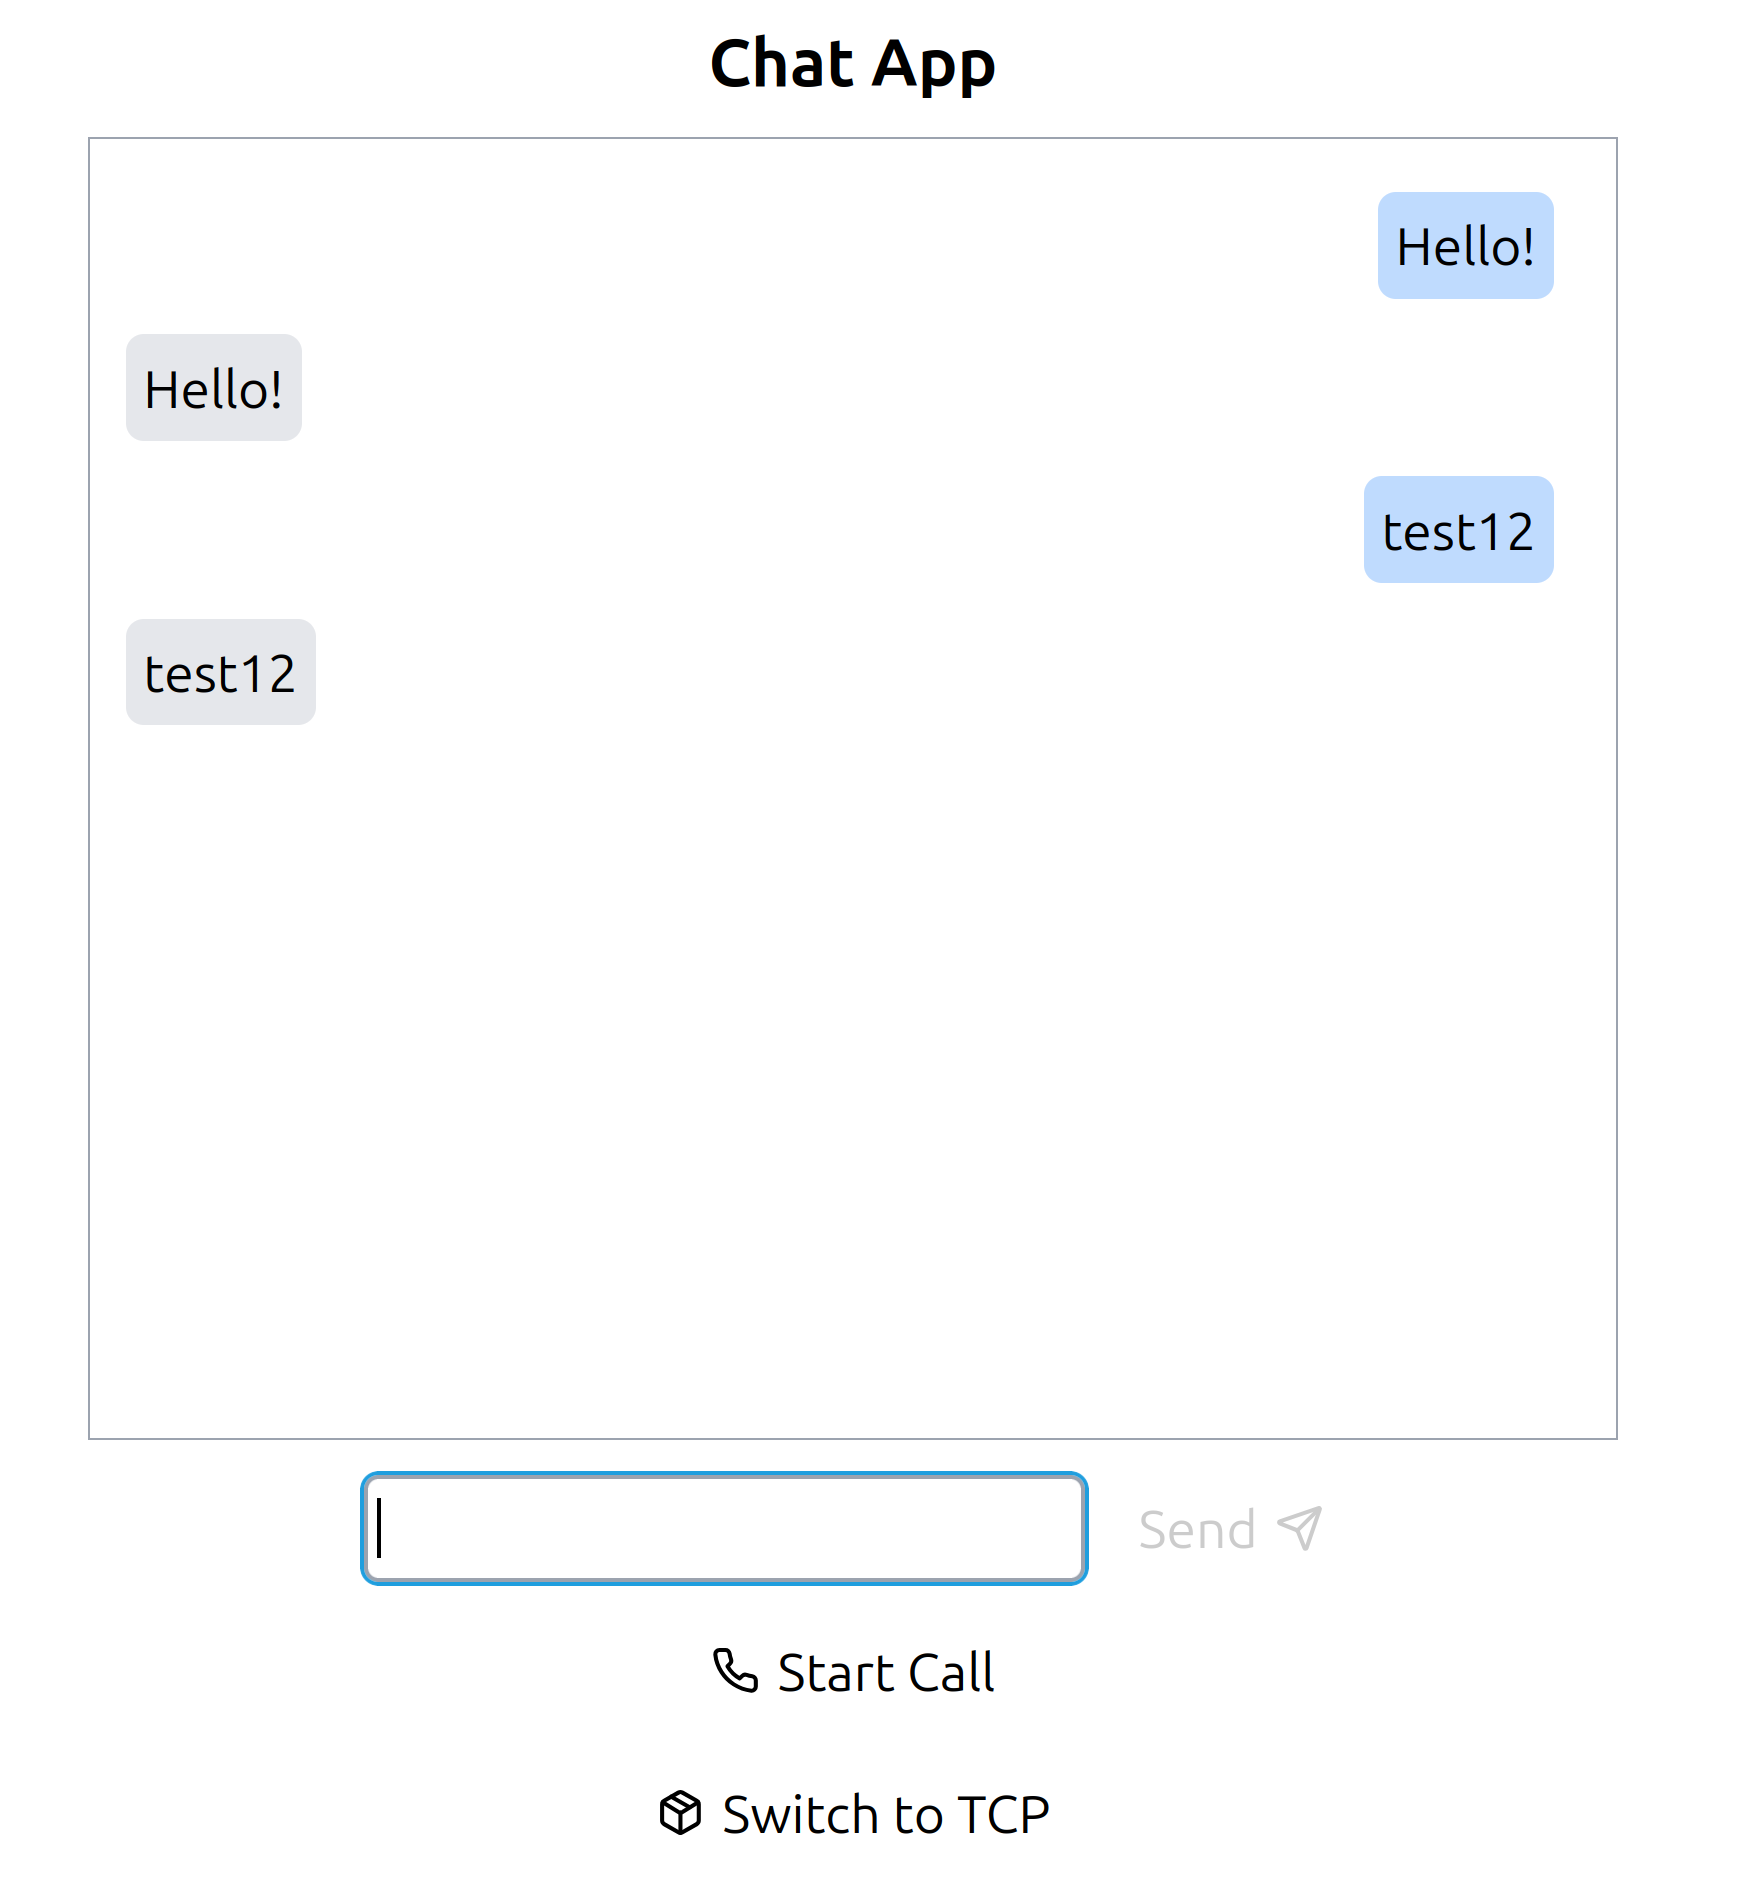
\includegraphics[width=0.8\textwidth]{chat1.png}
    \caption{Chat Application User Interface}
    \label{fig:chat1}
\end{figure}

\section{Wireshark packets}

\subsection{UDP Messages Packets}
\begin{figure}[h]
    \centering
    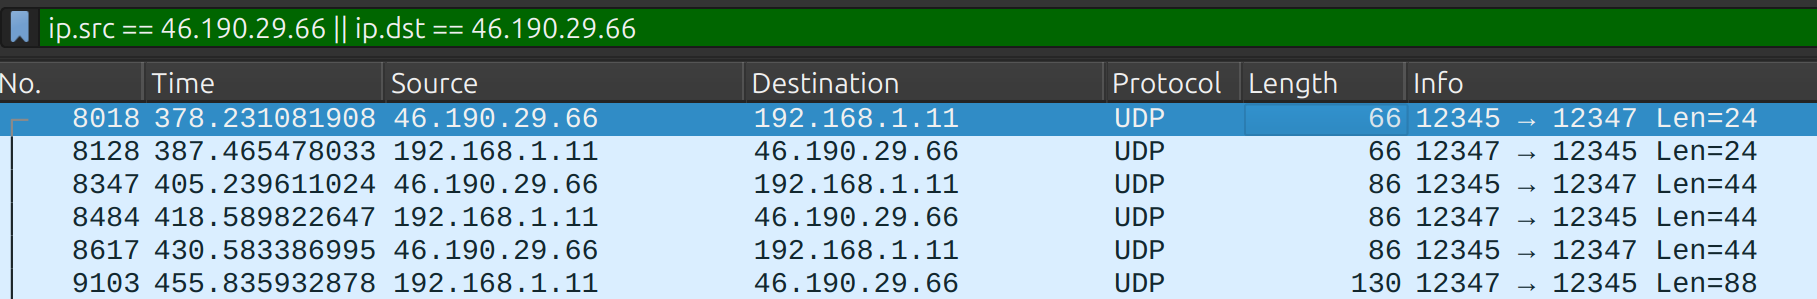
\includegraphics[width=0.8\textwidth]{udp-messages-1.png}
    \caption{UDP message packet exchanging with port forwarding}
    \label{fig:udp-messages-1}
\end{figure}

\begin{figure}[h]
    \centering
    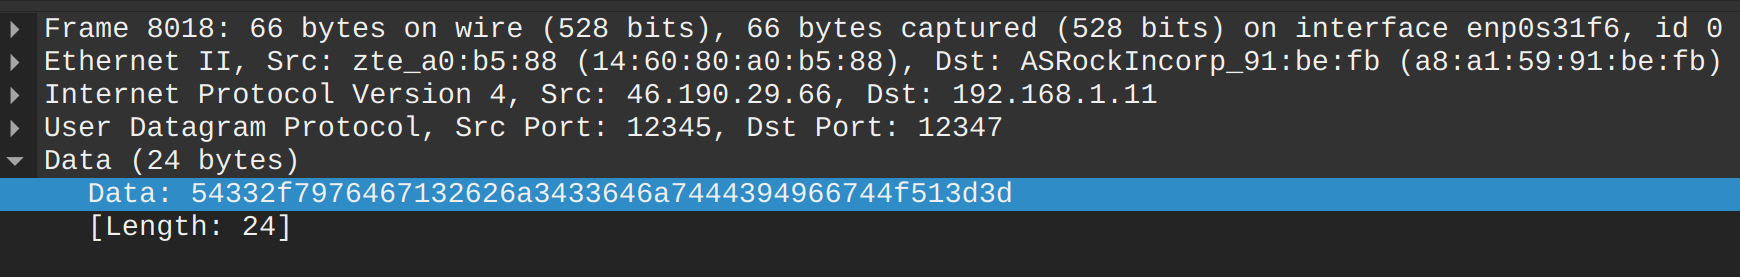
\includegraphics[width=0.8\textwidth]{udp-messages-2.png}
    \caption{UDP message packet (encrypted Payload marked)}
    \label{fig:udp-messages-2}
\end{figure}

\begin{figure}[h]
    \centering
    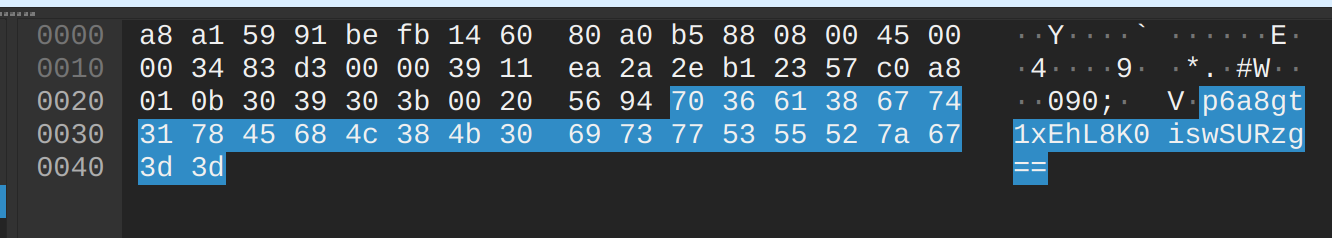
\includegraphics[width=0.8\textwidth]{udp-messages-3.png}
    \caption{UDP message packet (encrypted Payload marked)}
    \label{fig:udp-messages-3}
\end{figure}

We can see that the message is encrypted using the \texttt{AES} algorithm, which ensures the privacy of the communication.
The key used is \texttt{123456789ABCDEFG}.

Sending packets that are larger than 1024 bytes (encrypted) will not be received by the other peer, since the application only
uses a 1024 byte buffer. To send larger packets, the buffer size should be increased, or we need to split the message into smaller packets.




\subsection{UDP Voice Packets}

The voice packets are continuously sent and received between the two peers. The voice packets are sent in a continuous stream,
and the application uses a 1024 byte buffer to store the incoming voice data. The buffer is then played back to the user using the
\texttt{SourceDataLine} class.

\begin{figure}[h]
    \centering
    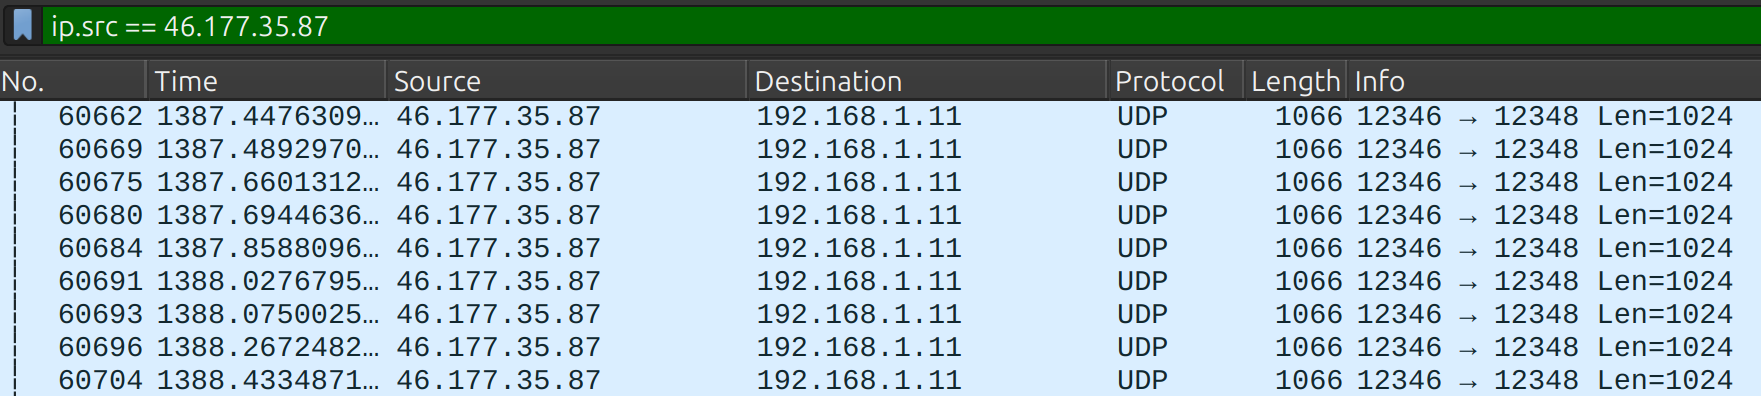
\includegraphics[width=0.8\textwidth]{udp-voice-1.png}
    \caption{UDP continuous voice packets}
    \label{fig:udp-voice-1}
\end{figure}

\begin{figure}[h]
    \centering
    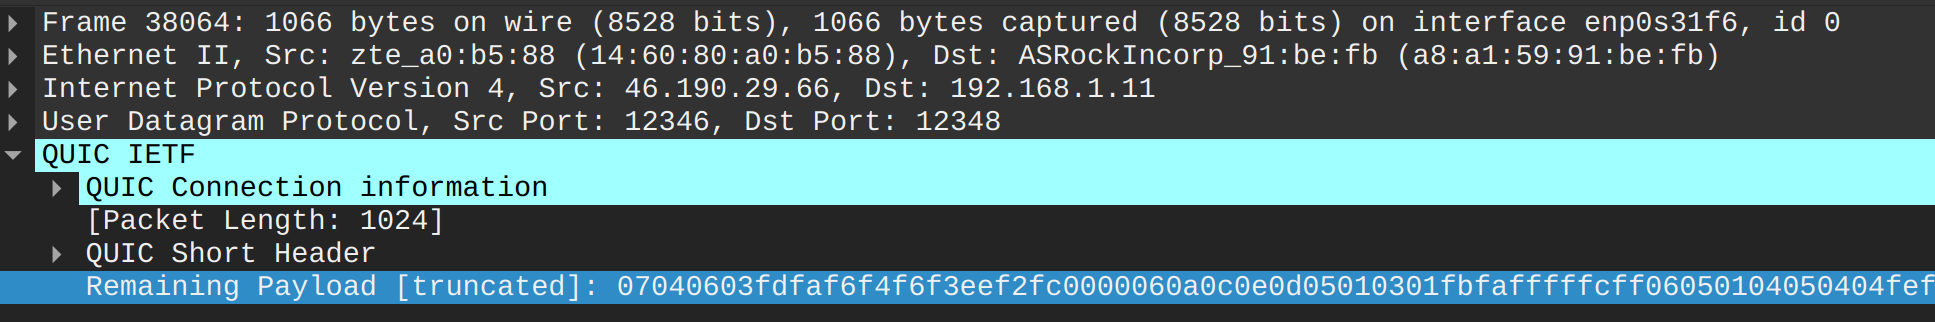
\includegraphics[width=0.8\textwidth]{udp-voice-2.png}
    \caption{UDP voice packet (Payload marked)}
    \label{fig:udp-voice-2}
\end{figure}

\begin{figure}[h]
    \centering
    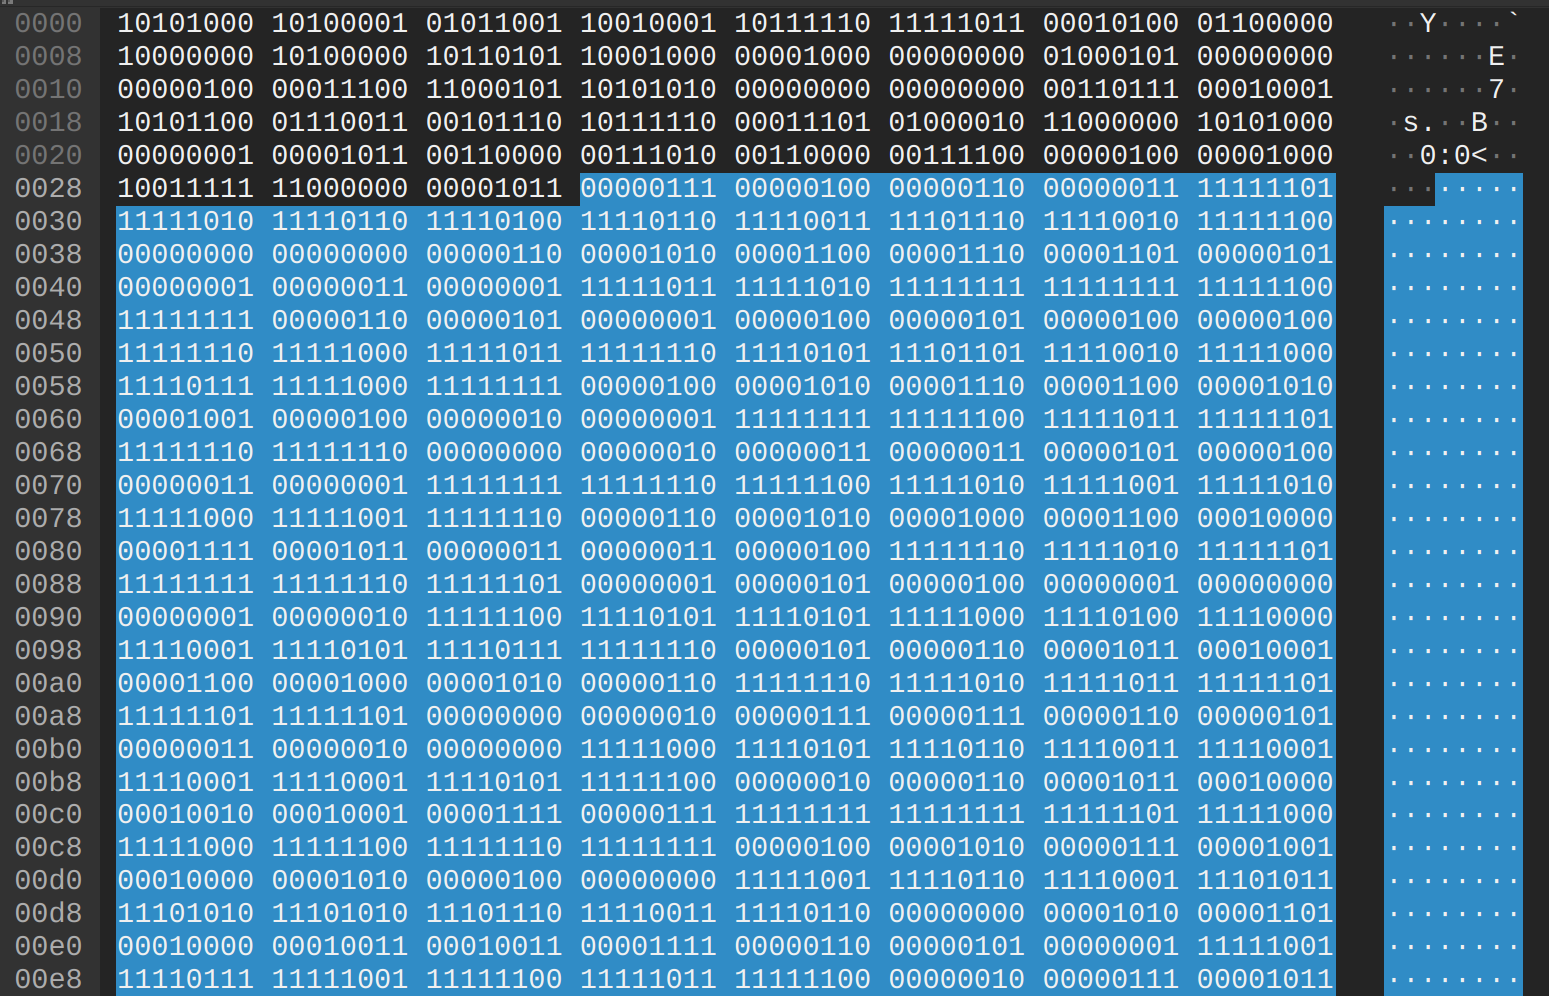
\includegraphics[width=0.8\textwidth]{udp-voice-3.png}
    \caption{UDP voice packet (Payload marked)}
    \label{fig:udp-voice-3}
\end{figure}


\section{References}
\begin{itemize}
    \item GitHub Repository: \url{https://github.com/siavvasm/CN2_AUTH_ChatAndVoIP}
\end{itemize}

\end{document}